\documentclass[../../main.tex]{subfiles}
\begin{document}

\begin{figure}[h!]
    \centering
    \includegraphics[width=\textwidth]{Comparison.png}
    \caption[Visual comparison of the algorithms]{A visual comparison of the four algorithms (from the top: PCISPH, two-scale, RTS, and finally our combined). The scene is \textit{double dam break with pillars} and the screen shots are taken at the times 0.3s, 1.6s, 3.3s, and 5.0s. }
    \label{fig:comparison}
\end{figure}

%%%%%%%%
\section{Results}
%%%%%%%%

As can be seen in tables \ref{table:gallery} through \ref{table:pillars}, our combined method has not shown the combined speedup of two-scale and RTS. In addition, our two-scale implementation has not given the speedup over PCISPH as shown in \citep{solenthaler2011two}. It has, in some cases, even taken twice as long as PCISPH. 

% "as expected"?
The RTS algorithm does not suffer from these slowdowns and show an increase in efficiency over PCISPH, as expected. We see that our combined algorithm gives a speedup over all other algorithms, except for in table \ref{table:doubledam}, the double dam break scene, where RTS is slightly faster. 

\begin{table}[]
\centering
\caption{Simulation results from the Gallery scene}
\label{table:gallery}
\begin{tabular}{llll}
\hline
Technique & Particle count      & Time (s) & Speedup \\ \hline
PCISPH    & 1.1M                & 54343.5  & -       \\
Two-scale & L: 140k H: 400-600k & 54923.5  & 0.989   \\
RTS       & 1.1M                & 47750.7  & 1.138   \\
Combined  & L: 144k H: 400-600k & 45385.8  & 1.197   \\ \hline
\end{tabular}
\end{table}


Visually, we see very few differences between the algorithms results, as is made clear in figure \ref{fig:comparison}. There is, of course, some difference between the L-area in the two-scale and combined algorithms, and the corresponding area in PCISPH and RTS. However, that is to be expected from the two-scale base algorithm, since the particle size differs outside the H-region. 

%%%%%%%%
\section{Discussion}
%%%%%%%%
The slowness of the two-scale simulation could be caused by a few differences from the original paper. Firstly, the resolution factor in our implementation is only 2, whereas in the two-scale paper it is in some tests set to 4. A resolution factor of 4 gives L-particles which are 64 times larger than the H-particles, reducing the total number of particles significantly. Secondly, our scenes and specifically the determination of the H-regions differs a bit. Our regions are up to 50\% of the whole simulation domain, and Solenthalers and Gross' seem to be around 25\% in most of the scenes. Because of the amount of H-particles, the overhead from certain calculations (create/delete H-particles, boundary handling, parent update) might outweigh the benefits of the two-scale method.

\begin{table}[]
\centering
\caption{Simulation results from the Double dam break with pillars scene}
\label{table:pillars}
\begin{tabular}{llll}
\hline
Technique & Particle count      & Time (s) & Speedup \\ \hline
PCISPH    & 950k                & 47172    & -       \\
Two-scale & L: 120k H: 300-570k & 117816   & 0.400   \\
RTS       & 950k                & 41841    & 1.127   \\
Combined  & L: 120k H: 300-570k & 40642.8  & 1.161   \\ \hline
\end{tabular}
\end{table}

\begin{table}[]
\centering
\caption{Time distribution over all parts in the combined algorithm}
\label{table:timedistribution}
\begin{tabular}{cccll}
\hline
\begin{tabular}[c]{@{}c@{}}Pre-Minor \\ L\end{tabular} & Determine Region & \begin{tabular}[c]{@{}c@{}}Pre-Minor\\ H\end{tabular} & Minor steps                 & Update Parent              \\ \hline
1.30\%                                                 & 17.70\%          & 7.40\%                                                & \multicolumn{1}{c}{70.60\%} & \multicolumn{1}{c}{3.00\%} \\ \hline
\end{tabular}
\end{table}


\begin{table}[]
\centering
\caption{Minor step time details}
\label{table:minordetails}
\begin{tabular}{ccccccc}
\hline
L                           & \multicolumn{5}{c}{H}                                                                                                                                                                                                                                                                      & Feedback             \\ \hline
\multicolumn{1}{c|}{}       & \multicolumn{5}{c|}{91.00\%}                                                                                                                                                                                                                                                                &                      \\ \cline{2-6}
\multicolumn{1}{c|}{7.90\%} & \begin{tabular}[c]{@{}c@{}}Update \\ neighborhood\end{tabular} & \begin{tabular}[c]{@{}c@{}}Update\\ density\end{tabular} & \begin{tabular}[c]{@{}c@{}}Prediction \\ correction\end{tabular} & \begin{tabular}[c]{@{}c@{}}Update vel \\ and pos\end{tabular} & \multicolumn{1}{c|}{Other}  & 1.10\%               \\ \cline{2-6}
\multicolumn{1}{l|}{}       & 36.60\%                                                        & 7.20\%                                                   & 46.00\%                                                          & 4.70\%                                                        & \multicolumn{1}{c|}{5.50\%} & \multicolumn{1}{l}{} \\ \hline
\end{tabular}
\end{table}

However, the most likely cause of the result is the behavior of the relaxed particles. During our implementation we had some difficulties with the boundary and relaxed H-particles for the two-scale algorithm and our combined algorithm, since they use the same calculations. It is possible that there still exists some problems which causes the particles to get incorrect densities which in turn requires more iterations in the prediction-correction loop. The fact that most of the $\Re_1$ regions exist near the border (as can be seen in figure \ref{fig:redarea}) further supports this theory.

We can also see in table \ref{table:timedistribution} and \ref{table:minordetails} that neither update parent nor feedback calculations, two-scale specific steps, are taking a lot of time. The determine region part alone takes a notable amount of time but this is likely due to bad memory management. Currently we de-allocate and allocate new memory every time we remove or create new H-particles. A better memory management scheme could reuse memory and thus alleviate the overhead of memory allocation and improve performance by reducing memory fragmentation. This is, however, probably not the cause of the two-scales slow results due to its significant difference compared to our combined algorithm, which uses the same memory management. 

\begin{table}[]
\centering
\caption{Simulation results from the Double dam break scene}
\label{table:doubledam}
\begin{tabular}{llll}
\hline
Technique & Particle count      & Time (s) & Speedup \\ \hline
PCISPH    & 950k                & 45486.4  & -       \\
Two-scale & L: 120k H: 300-500k & 105931   & 0.429   \\
RTS       & 950k                & 40519    & 1.123   \\
Combined  & L: 120k H: 300-500k & 42342.4  & 1.074   \\ \hline
\end{tabular}
\end{table}

We see that our combined algorithm on average is faster than RTS and PCISPH, despite that the two-scale results shows much longer simulation time than PCISPH. This indicates that if our two-scale implementation gave the same speed up as in the original paper, we would see a large speed up in our combined algorithm as well. 

One reason to why RTS is faster in the Double dam break scene could be that because there are no pillars in the H-region, fewer particles are determined to belong to $\Re_1$, since less sudden impacts occur. This, in turn, could result in the particles getting slightly incorrect positions due to the reduction of calculations performed on them. The result would be that more iterations of the prediction correction loop would have to be performed, and as can be seen in \ref{table:minordetails} that is a large part of the algorithm. Thus, ultimately, making the combined simulation take more time than RTS.

Also worth noting is that each test was only performed once, and therefore there is a possibility that some results might have been compromised by external influences. However, this does not explain the long simulation time of the two-scale algorithm, since we see the same slowness for all three scenes. 

\begin{figure}[h]
    \centering
    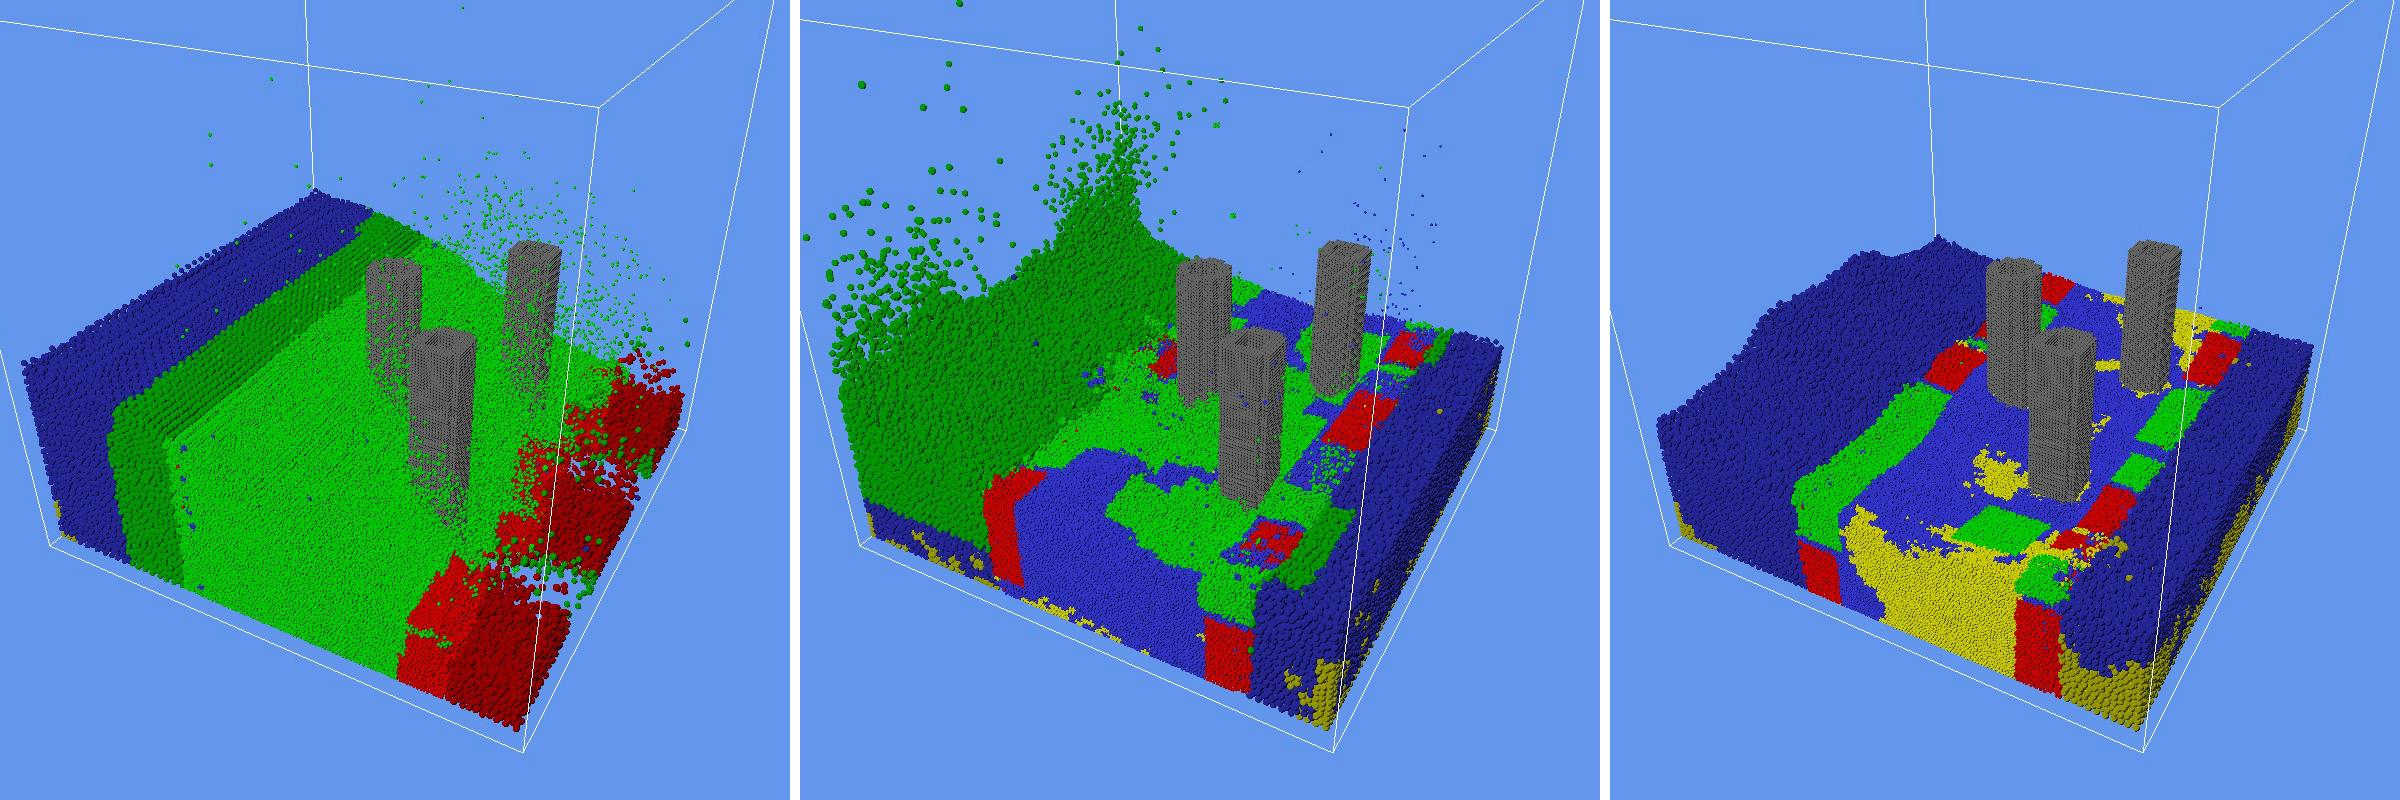
\includegraphics[width=\textwidth]{RedArea.png}
    \caption[Lower time step along the border]{The $\Re_1$ area (colored red) is prominent along the border between H and L, even when the particles should not be experiencing large forces, like in the middle of the yellow $\Re_4$ region. }
    \label{fig:redarea}
\end{figure}

\end{document}